\section{Validation}\label{sec:validation}

This section states how the results of Section~\ref{sec:results} are known to be computed correctly: by closed forms independent of the engine's
numerics, by two implementations held equal, by a stochastic re-derivation of the balance, by a units check on every prediction, by tests that plant
defects, and by reconciliation with the published calibration. None of these is a model judging a model.

\subsection{Closed forms and conservation}\label{sec:val-oracles}

Three oracles in \texttt{pipeline/\allowbreak{}oracles.py} compute quantities by closed form, independently of the engine's numerics, and the tests compare them with
the engine. The Rosin-Rammler passing at the characteristic size must equal $1-1/e$ (Equation~\eqref{eq:rr} at $x=x_{63}$); the Bond energy of a reduction
from $F_{80}$ to $P_{80}$ must equal its closed form (Equation~\eqref{eq:bond}) evaluated directly; and the mass of every baked product must sum to the
feed's within the solver's closure. The closure itself is reported in every trace before the product is renormalised: at S01 it is $3.3\times10^{-16}$, a few
units of round-off for a sum of $28$ terms, and the conditioning proxy is $1.517$, so the system is far from the threshold of $10^{6}$ at which a point is
flagged. The breakage matrix of every case is strictly lower triangular with columns summing to one, which, by the derivation of
Section~\ref{sec:m-whiten}, is what makes the balance conserve mass. The trends that the engine must reproduce are tested as inequalities: a tighter setting
gives a finer product, a wider throw a coarser product with a higher capacity, the capacity is unimodal in speed, and the classification is monotone.

\subsection{Two engines held equal}\label{sec:val-parity}

The Python and TypeScript engines are held to a shared reference file of $\nrefpoints$ operating points, which covers the five machine classes, $27$ points with the
calibrated switch on, and $107$ choke, $13$ pass-through and $4$ invalid points. For every point every result field and every feature vector of the two learned models must agree
within $10^{-9}$ relative; the largest relative difference measured over the file is $\refworst$, about $10^{4}$ units of round-off, which is
what two implementations of the same operations in the same order produce. A second test re-runs every baked case in TypeScript and compares it with the
committed trace to the six significant digits the trace is written with, so a change to either engine that is not replicated in the other fails both a
unit test and a build. The drift projection has its own shared table of $45$ rows, reproduced on both sides to $10^{-6}$~mm, and the model encodings of
the browser are checked against the same reference, float32 rounding included.

\subsection{The balance re-derived by a particle-replacement walk}\label{sec:val-walk}

The Whiten product is the expectation of a simple stochastic process: parcels of feed enter the chamber with the feed proportions; in each pass a class-$j$
parcel is nipped with probability $c_j$; the parcels not nipped leave as product, and the nipped ones of class $j$ are redistributed over the finer classes
by the column $\mathrm B_{\cdot j}$ and enter the next pass, until none is inside. This is the particle-replacement rule of discrete-element crusher models
reduced to counts of parcels per class. If $\mathbf n^{(m)}$ is the expected number of parcels inside at pass $m$ per unit of feed, then
$\mathbf n^{(0)}=\mathbf f$ and $\mathbf n^{(m+1)}=\mathrm B\mathrm C\,\mathbf n^{(m)}$, so the expected product and the expected number of nips per parcel are
\begin{equation}
\mathbb E[\mathbf p_{\mathrm{walk}}] = (\mathrm I-\mathrm C)\sum_{m\ge0}(\mathrm B\mathrm C)^m\,\mathbf f = (\mathrm I-\mathrm C)(\mathrm I-\mathrm B\mathrm C)^{-1}\mathbf f,
\qquad
\mathbb E[\nu_{\mathrm{walk}}] = \mathbf 1^{\top}\mathrm C\,(\mathrm I-\mathrm B\mathrm C)^{-1}\mathbf f ,
\label{eq:walk}
\end{equation}
the Neumann series converging because $\mathrm B\mathrm C$ is nilpotent (strictly lower triangular). A walk of $N$ parcels therefore estimates the Whiten
product with a Monte Carlo error that should fall as $N^{-1/2}$. The product's function \texttt{replacement\_walk} implements this walk; the figure script of
the report runs it on the chamber of case S01 (assembled by \texttt{assemble\_chamber}) for $100$ to $100{,}000$ parcels with five seeds each, and compares it
with \texttt{evaluate}. These numbers are computed by the committed script \texttt{figures/\allowbreak{}make\_figs.py} calling the product's code, and are not stored in a
product artifact. Figure~\ref{fig:replacement}(a) shows the largest difference per class between the walk and the Whiten product: $0.060$ at $100$ parcels
and $0.0020$ at $100{,}000$, along a slope of $-1/2$. Figure~\ref{fig:replacement}(b) shows the mean number of nips per parcel converging to the value
$\sum_ic_ix_i=0.8858$ of Equation~\eqref{eq:nips}. The walk and the solve are two derivations of the same model, so their agreement validates the
implementation of the solve, not the physics of the model.

\begin{figure}[!t]
\centering
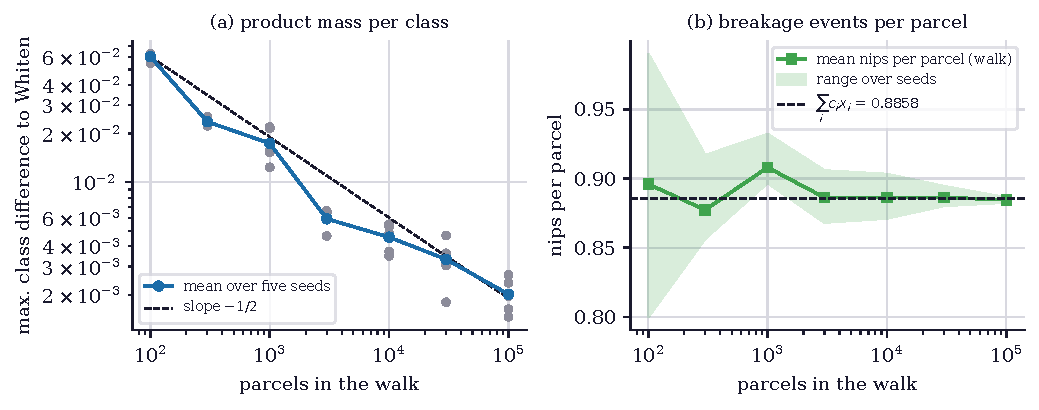
\includegraphics[width=\textwidth]{fig-replacement.pdf}
\caption{The particle-replacement walk on the chamber of case S01 against the Whiten solve, computed by the report's figure script with the product's engine
code: (a) largest difference per size class between the walk's product and the Whiten product against the number of parcels (five seeds, grey; mean, blue;
slope $-1/2$, dashed); (b) mean nips per parcel against the expectation $\sum_i c_i x_i$.}
\label{fig:replacement}
\end{figure}

\subsection{Units of every prediction}\label{sec:val-units}

Every prediction of a case must live in the units of its observable. For an observable with range $[L,H]$, the prediction $\hat y$ must be finite and satisfy
\begin{equation}
L - (H-L) \ \le\ \hat y\ \le\ H + (H-L),
\label{eq:units}
\end{equation}
a range widened by one full range on each side. For the three measured observables of a real case (throughput, power and $f_{80}$) the range is that of the
ten surveys; for every other observable, and for every observable of a circuit case, it is the physical domain the engine declares: sizes from $0$ to the
$256$~mm top of the grid, a reduction ratio from one to the ratio of the top to the finest edge, a throughput from $0$ to ten times the reference capacity of
the machine class, a power from $0$ to $3000$~kW, and a specific energy from $0$ to $20$~kWh/t. The check runs inside the bake and again over the shipped
artifacts in continuous integration, with the standard library only. It is a units check, not an accuracy check: a poor prediction inside the widened range
passes, which is intended; and it cannot catch a swap between two observables whose ranges overlap numerically (a power and a throughput on the HP500 range),
which the per-case expected ranges and a cross-case test catch instead. A separate script checks that the engine's constants carry their units.

\subsection{Tests that plant defects}\label{sec:val-adversarial}

Several results are guarded by tests that plant the defect they guard against. An absurd target planted in one survey must move every other fold's prediction
and not its own, for every fitted predictor including the line and CrusherBayes, which proves that no fold sees its held-out survey. The label-shuffle control
must not beat the backbone. Swapping a model slot to its baseline must keep the contract, so that the web never shows a learned number when the bundle is
invalid. A short chain must be recorded as not converged. The CrusherBayes document must be byte-identical whatever the number of worker processes, and the
integrated-out discrepancy of Equation~\eqref{eq:cbmarginal} is checked against a Monte Carlo of the model in Equation~\eqref{eq:cbmodel}. Every committed
document validates against its schema on both sides of its contract, the readiness document must be current with the catalog, a planted document that breaks
a cross-field rule must be refused, and a guard of the test suite fails any test that would rewrite the committed artifacts.

\subsection{Reconciliation with the published calibration}\label{sec:val-published}

The calibrated lane is reconciled with the published calibration in two ways. The engine with the published constants reproduces the measured feed rates of
the ten surveys with an in-sample MAPE of $11.55\%$, and its capacity base refit per fold stays close to the published value: the posterior mean of the capacity
base fitted to all ten surveys is $646.3$~t/h against the published $647$~t/h. The published power constants do not reconcile with the Bond draw ($47.58\%$
in sample), which the source itself explains, because they belong to a different net power. The paper's own error figures are printed as figures and the
publisher page could not be opened, so no comparison of the held-out errors with an in-sample error band of the paper is made; the held-out error is set
beside the in-sample error of the same backbone computed by the product. A re-transcription of the published survey table that disagreed with
the committed file would remove the real lane from a build until the table is corrected.
